\chapter{Results and Analysis}
The numerical results are displayed in this chapter for both parachute simulation and DNS of cloud entrainment process. In each part, the experimental setups are firstly introduced, and then the numerical results and quantitative analysis are presented.

\section{Results for parachute simulation}
This section aims to demonstrate the improvements and features of the new parachute model. Firstly, the experimental setup are introduced including the domain size, boundary conditions, and the initialization of parachute canopy and flow field. Then the turbulent-viscosity models are incorporated to the current code and compared with the laminar-version simulation. In the meanwhile, we try to investigate the new porosity model, and compare its effects with the previous non-porous parachute. Finally, the collision handling modules are applied to simulate the fabric collision and folding procedure.
 
\subsection{Experimental setup}
The experiments are carried out in a wind tunnel, which is set to be $14m\times14m\times 40m$ as default with constant velocity at the inlet, outflow boundary condition with pressure $p = 0$ $Pa$ at the outlet, and periodic boundary condition for the rest of faces. In some situations, the periodic boundary condition can be replaced by the non-slip boundary condition or wall boundary condition. The domain size may also change for some specific reasons. As for the parachute types, we consider several descending round canopies: C-$9$, G-$11$, G-$12$, G-$14$ and T-$10$. 

The C-$9$ type parachutes are used in the Advanced Concept Ejection Seat (ACES) in all current U.S. jet fighters and personal parachutes in cargo airplanes. It has $8.5m$ nominal diameter, $28$ number of gores, $7m$ suspension lines. 
The G-$11$ $100$-feet parachute is heavy capacity cargo parachute designed primarily for used in the aerial delivery of vehicular and bulk-type platform loads. It has $30.3m$ diameter, $120$ suspension lines with length of $10.6m$. Each $10$ of the consecutive suspension lines are connected to a suspension riser, and thus giving $12$ suspension risers with length of $18.28m$. These suspension risers are further evenly divided into three suspension riser assemblies terminating in three riser attaching loops. 
The G-$12$ $64$-feet cargo parachute is designed for medium capacity use with the A-$22$ air delivery cargo bag. It has the similar structure as G-$11$ while with $64$ suspension lines of $15.5m$ and $8$ risers of $18.2m$. 
The G-$14$ $34$-feet cargo parachute provides the capability to deliver non-fragile supplies and equipment using low-velocity air delivery method. It can also be assembled to a cluster of three to support payloads up to $1500$ $lbs$. It has $32$ suspension lines of length $8.3m$ with two risers. 
The T-$10$ $35$-feet personnel parachute is designed for combat mass-assault airborne operations and training. It is a parabolic-shape and has a nominal diameter of $10.7m$ with $30$ suspension lines. The technical specifications for these canopies are listed in \Table{parachute_specification}, and \Figure{init_parachutes} illustrates the scales and initial shapes of different types of parachutes. The strings attached to the canopies of G-$11$ and G-$12$ reflect the result of combined effects of suspension lines and riser lines.
\begin{table}
\centering
\begin{tabular}{lcccc}
\hline\hline
Type   & Diameter & Shape 		  & Suspensions        & Risers \\
\hline
C-$9$  & $8.5m$   & flat circular & $28\times 7m$     & none   \\
G-$11$ & $30.3m$  & flat circular & $120\times 10.6m$ & $12\times 18.2m$ \\
G-$12$ & $19.5m$  & flat circular & $64\times 15.5m$  & $8\times 18.2m$ \\
G-$14$ & $10.3m$  & flat circular & $32\times 8.3m$   & $2\times 0.76m$ \\
T-$10$ & $10.7m$  & parabolic     & $30\times 8.5m$   & $2\times 0.76m$\\
\hline
\end{tabular}
\caption{The technical specifications of parachutes}\label{parachute_specification}
\end{table}

\begin{figure}[!htbp]
\centering
\includegraphics[width=\textwidth]{Figures/init_parachutes.jpg}
\caption{Initial shapes of parachutes, from left to right are C-$9$, T-$10$, G-$14$, G-$12$, G-$11$.}\label{init_parachutes}
\end{figure}

The computational mesh consist of two parts: the Eulerian mesh of fluid field and Lagrangian mesh of the parachute canopy. The fluid field is computed in a three-dimensional rectangular grid with uniform grid spacing. Various resolutions are tested depending on the domain size and the required accuracy. The canopies' mesh is generated by CGAL $2$D triangulations package \cite{CGAL_Triangulation} based on the constrained Delaunay triangulation. The computational mesh of T-$10$ parachute is displayed in \Fig{T10-mesh} for illustration.
\begin{figure}[!htbp]
\centering
\includegraphics[width=0.3\textwidth]{Figures/T10-mesh-top.png}
\includegraphics[width=0.3\textwidth]{Figures/T10-mesh-front.png}
\includegraphics[width=0.3\textwidth]{Figures/T10-mesh-rear.png}
\caption{Initial mesh of T-$10$ canopy.}\label{T10-mesh}
\end{figure}

Two major settings have been applied in the wind tunnel: the drop test and the fixed-end test. In the drop test, the parachute is released at the top of the wind tunnel from either folded or unfolded shapes, and then the parachute freely falls in the tunnel until it hits the ground. This experiment aims to simulate the inflation stage of the parachute falling and study the factors affecting this procedure. The settings of drop test is close to a real situation, it, however, may terminate before the parachute reaching the stable state. Instead of free falling, the fixed-end test fixes one end of the parachute, and let the wind blow into the tunnel to inflate the canopy. This test can be used to measure the drag force on the canopy and is able to run arbitrarily long until the drag becomes stable.
  
\subsection{Turbulent-viscosity models}
The Reynolds number around a full-size parachute usually exceeds several millions, and hence the fluid flow has to be treated as turbulence \cite{Johari05}. The turbulent-viscosity models is one of many approaches to simulate the turbulent effects. In the current parachute simulation, a two-equation model has been developed attempting to duplicate several features during the turbulence-parachute interactions. The principle of the two-equation model is to modify the viscosity coefficient in the Reynolds-averaged Navier-Stokes equation, so as to approximate the effects of Reynolds stresses. The turbulent viscosity is computed from turbulence quantities such as $k$ and $\varepsilon$, which are solved from a couple of transport equations. In this section, three types of $k-\varepsilon$ model, standard, Re-Normalisation Group (RNG), and realizable turbulence model are investigated in the parachute drop test, and meanwhile compared with the simulation results without using turbulence model, in which the viscosity is a constant. The velocity magnitude and turbulence viscosity for each model are recorded. 

\Fig{turbulent_visc_vel_3ms} shows the velocity magnitude and turbulent viscosity for different models at the same time frame. When the inlet velocity is $3m/s$, it shows that all the $k-\varepsilon$ models produce similar flow patterns, and they also resemble the pattern in the simulation without using turbulence model. However, the standard model tends to predict higher velocity magnitude than the RNG model and Realizable model and the flow patterns near the parachute vent are significantly different. As for the turbulent viscosity, the standard model resembles the pattern of RNG model while its numeric value is one order of magnitude larger. It is interesting to see that, in the realizable model, the viscosity after the parachute canopy is significantly smaller than the other two models. This is because the realizable model predicts higher turbulence dissipation rate $\varepsilon$ in the parachute wake, and thus the viscosity quickly decreases according to the formula $\mu_{t} = C_{\mu}\rho k^2/\varepsilon$.

\Fig{turbulent_visc_vel_10ms} shows the same test, yet with inlet velocity $10m/s$. It is reasonable that the parachutes are subjected to stronger drag force than the case of $3m/s$, and hence falls much slower. The Realizable model still predicts the smallest value of the viscosity in the wake of the parachute. However, since the inflow velocity increases, the kinetic energy and dissipation rate produced at the inlet are able to propagate further and dominate the viscosity field. As the parachute falls and interacts with the inlet flow, it pushes the turbulent viscosity field away to each side and generates vortex-like pattern \cite{Johari05}.

\Fig{turbulent_visc_vel_15ms} displays the velocity and viscosity field with inlet velocity $15m/s$. This test gives a real turbulence field, and therefore the predictions of the three models are expected to be reasonable. The viscosity field predicted by the RNG model resembles the standard one but with more details in the wake, while the realizable model produces a completely different viscosity field. This field results in a more chaotic velocity field than the other two cases. We also notice that using turbulence model makes the parachute drop significantly faster than the case without turbulence model. This can be explained by the fact that the turbulence viscosity plays as a friction between fluid elements, and hence reduce the velocity magnitude and the drag force.

In summary, the standard $k-\varepsilon$ model assumes that the flow is fully turbulent, and the effects of molecular viscosity are negligible. This model was demonstrated to work fairly well for a wide range of wall-bounded and free shear flows. However, since the parachute canopy prevents the flow from passing through and the flow behind the parachute is less-turbulent when the inlet velocity is small, the standard model tends to overestimate the turbulent viscosity in the parachute wake. The RNG model is integrated to obtain an accurate description of how the effective turbulent transport varies with the effective Reynolds number, allowing the model to better handle low-Reynolds-number and near-wall flows. The RNG model is expected to be more responsive to the effects of rapid strain and streamline curvature than the standard model. Hence in the rapidly strained flows, it yields a lower turbulent viscosity than the standard model. The Realizable model is proposed by satisfying certain mathematical constrains on the normal stresses, consistent with the physics of turbulent flows. It is believed that the modified form of the equation for $\varepsilon$ better represents the spectral energy transfer. The performance of the model has been found to be substantially better than that of the standard model.

\begin{figure}[!htbp]
\centering
\includegraphics[width=0.24\textwidth]{Figures/c9-vel-std-3ms.jpg}
\includegraphics[width=0.24\textwidth]{Figures/c9-vel-rng-3ms.jpg}
\includegraphics[width=0.24\textwidth]{Figures/c9-vel-real-3ms.jpg}
\includegraphics[width=0.24\textwidth]{Figures/c9-vel-lam-3ms.jpg}\\
\includegraphics[width=0.24\textwidth]{Figures/c9-vis-std-3ms.jpg}
\includegraphics[width=0.24\textwidth]{Figures/c9-vis-rng-3ms.jpg}
\includegraphics[width=0.24\textwidth]{Figures/c9-vis-real-3ms.jpg}
\includegraphics[width=0.24\textwidth]{Figures/c9-vis-lam-3ms.jpg}
\caption{Velocity magnitude and turbulent viscosity for C-$9$ parachute using different turbulent models at the same time frame. The inlet velocity is $3m/s$. The figures in the upper row displays the velocity magnitude and the figures in the lower row shows the turbulent viscosity.}
\label{turbulent_visc_vel_3ms}
\end{figure}

\begin{figure}[!htbp]
\centering
\includegraphics[width=0.24\textwidth]{Figures/c9-vel-std-10ms.jpg}
\includegraphics[width=0.24\textwidth]{Figures/c9-vel-rng-10ms.jpg}
\includegraphics[width=0.24\textwidth]{Figures/c9-vel-real-10ms.jpg}
\includegraphics[width=0.24\textwidth]{Figures/c9-vel-lam-10ms.jpg}\\
\includegraphics[width=0.24\textwidth]{Figures/c9-vis-std-10ms.jpg}
\includegraphics[width=0.24\textwidth]{Figures/c9-vis-rng-10ms.jpg}
\includegraphics[width=0.24\textwidth]{Figures/c9-vis-real-10ms.jpg}
\includegraphics[width=0.24\textwidth]{Figures/c9-vis-lam-10ms.jpg}
\caption{Velocity magnitude and turbulent viscosity for C-$9$ parachute using different turbulent models at the same time frame. The inlet velocity is $10m/s$. The figures in the upper row displays the velocity magnitude and the figures in the lower row shows the turbulent viscosity.}
\label{turbulent_visc_vel_10ms}
\end{figure}

\begin{figure}[!htbp]
\centering
\includegraphics[width=0.24\textwidth]{Figures/c9-vel-std-15ms.jpg}
\includegraphics[width=0.24\textwidth]{Figures/c9-vel-rng-15ms.jpg}
\includegraphics[width=0.24\textwidth]{Figures/c9-vel-real-15ms.jpg}
\includegraphics[width=0.24\textwidth]{Figures/c9-vel-lam-15ms.jpg}\\
\includegraphics[width=0.24\textwidth]{Figures/c9-vis-std-15ms.jpg}
\includegraphics[width=0.24\textwidth]{Figures/c9-vis-rng-15ms.jpg}
\includegraphics[width=0.24\textwidth]{Figures/c9-vis-real-15ms.jpg}
\includegraphics[width=0.24\textwidth]{Figures/c9-vis-lam-15ms.jpg}
\caption{Velocity magnitude and turbulent viscosity for C-$9$ parachute using different turbulent models at the same time frame. The inlet velocity is $15m/s$. The figures in the upper row displays the velocity magnitude and the figures in the lower row shows the turbulent viscosity.}
\label{turbulent_visc_vel_15ms}
\end{figure}
\subsection{Porosity model}
Two sets of numerical tests are carried out to validate the porosity model 
and its underlying numerical method. 
The first set of tests is designed to study a steady incompressible flow
through a porous interface. The purpose of this numerical test is to 
verify the implementation of our method. The pressure drop is expected to appear exactly 
at the interface position as the model described in \Eq{jumpcond}. 
The computational domain is set to be $4 m\times
0.4 m\times 0.4 m$ in the $x$, $y$, $z$ directions, respectively. The velocity is
driven by an inflow with a parabolic profile: 
\begin{equation}
\mathbf{u}(x=0,y,z) = [16U_{max}yz(L_y - y)(L_z - z)/(L^2_yL^2_z),0,0]
\end{equation} 
where $U_{max}$ is the maximum velocity at the center of the
inlet, $L_y$ and $L_z$ are the width of the channel in $y$ and $z$ directions. 
An outflow boundary condition together with the pressure $p = 0 Pa$ is applied to 
the outlet at $x = 4 m$ and a non-slip boundary condition of $\mathbf{u} = \mathbf{0}$ 
is imposed for the remaining faces. The porous interface is orthogonal to the streamline 
of flow and is placed at $x = 2m$. The coefficients in equation \Eq{jumpcond} are set as 
$\alpha = 10 kgm^{-1}s^{-1}$ and $\beta = 0 kgm^{-2}$.
The profiles of velocity and pressure at different positions are shown in \Fig{fig:test1_profile}.  	

\begin{figure}[H] \centering
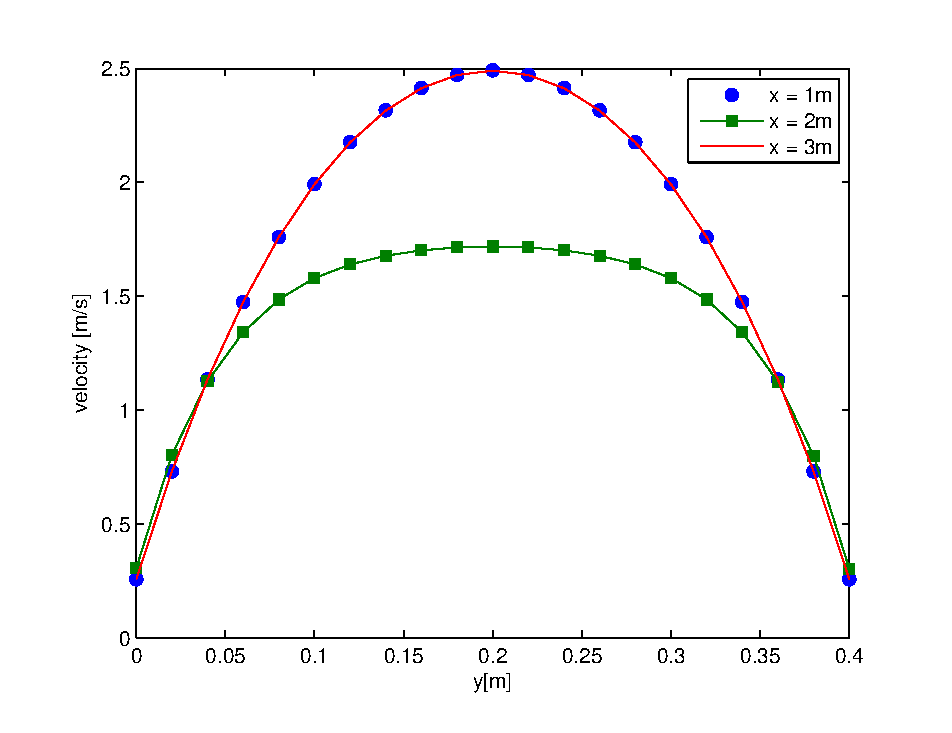
\includegraphics[width=0.49\columnwidth]{Figures/ucrs_profile}
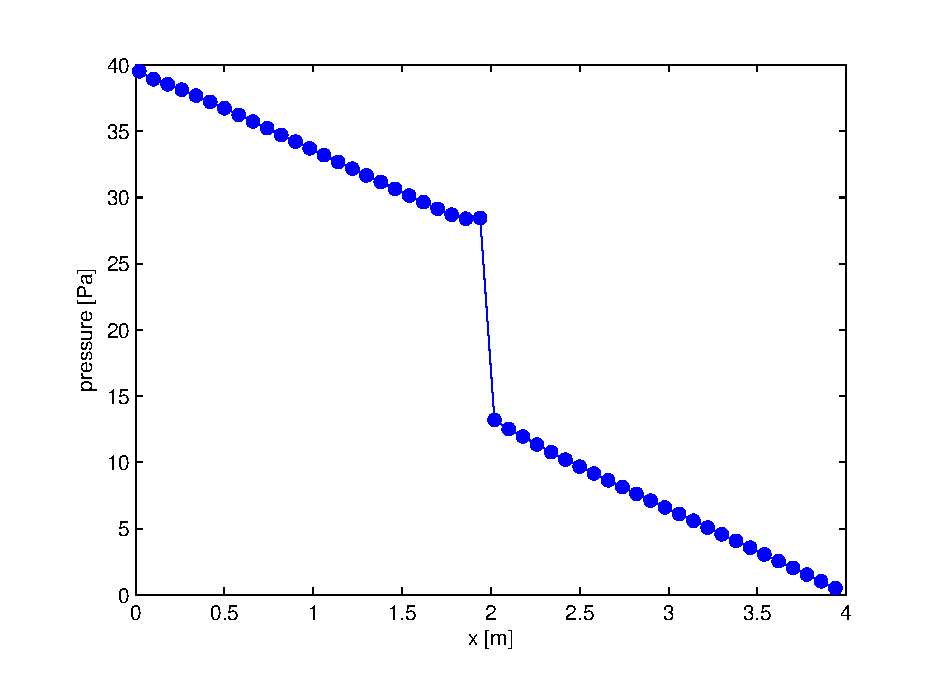
\includegraphics[width=0.49\columnwidth]{Figures/p_profile} \caption{(left)
Streamwise velocity profile at different sliced cross section and 
(right) pressure along a axial direction with $y = 0.2 m, z = 0.2 m$. The plot 
shows the velocity changes its profile as the fluid passes through the interface. 
The pressure drop at the interface is well captured.} 
\label{fig:test1_profile} 
\end{figure}

In the second set of tests, a full-scale model is used to simulate the response
of a realistic fabric surface in the channel flow.  The boundary conditions of
the computational domain are the same as the ones in the first test except that
the domain size is $30 m\times 10 m\times 10 m$. The elastic fabric surface located
at $x = 5 m$ is from the spring-mass model described in
\cite{Shi2015Verification}. Thus the surface can be stretched or compressed due
to the pressure drop at the interface.  The fabric tested in the simulations
resembles the properties of MIL-C-7020 type III fabric \cite{ewing1978recovery}
with density $533.77 kgm^{-3}$, Young's modulus $0.4309 Gpa$. The values of viscous 
and inertial parameters are $\alpha = 162 kgm^{-1}s^{-1}$ and 
$\beta = 48.82 kgm^{-2}$, which are calculated by fitting 
the experimental data using a quadratic function.
The permeability velocity and the pressure drop are 
measured by taking the average of the velocity and pressure drop over the entire surface. 
By imposing different values of inflow velocity, the functional relationship 
between these two variables can be obtained. We approximate the experimental data in \cite{ewing1978recovery} with formula $[p]_{\Gamma} = \alpha U_n + \beta U_n^2$ 
and use it as the reference solution. The results presented in \Fig{fig:curve} 
show that our model can successfully reproduce the quadratic relationship observed in the experiments. 

\begin{figure}[!htbp] \centering
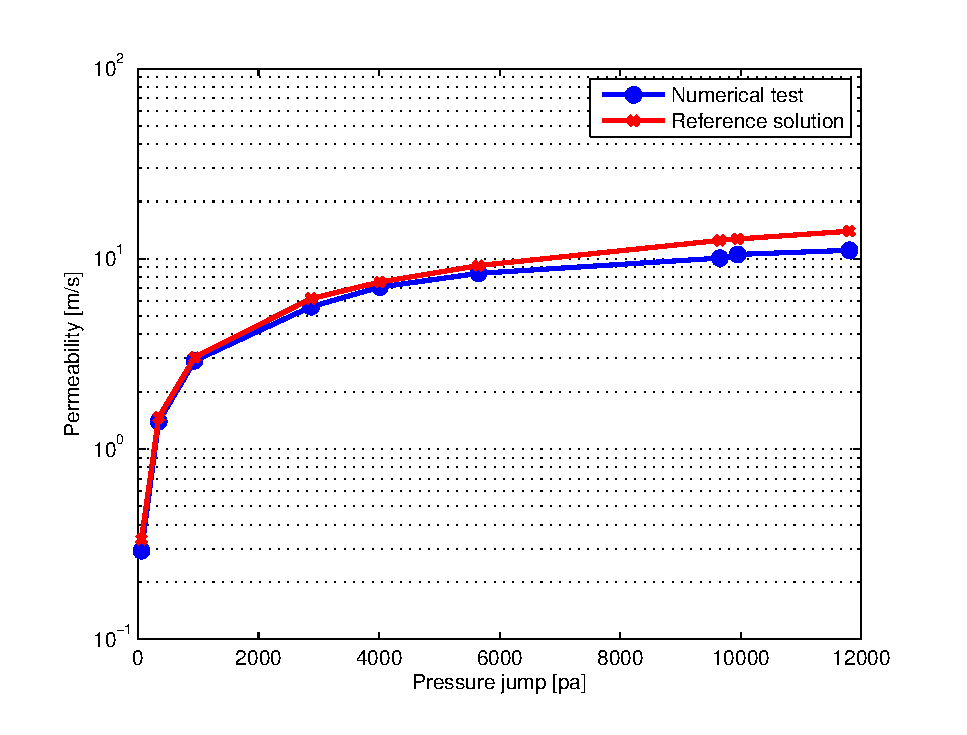
\includegraphics[width=1.0\columnwidth]{Figures/curve} \caption{Plot 
of permeability velocity vs. pressure drop for the test case. 
The numerical results show that there 
is a quadratic relationship between the permeability velocity and
pressure drop. Such relationship is observed in the experiment (red line)} 
\label{fig:curve} \end{figure}

In this section, we report our application of
the porosity model to the parachute simulation and compare the drag force with 
the same force as in the impermeable cases. The drag forces and drag
coefficients are calculated with varying freestream velocity at the inlet.
The drag measurement is carried out in a wind tunnel setting on G11 cargo
parachute with its nominal diameter $10 m$ and point of load fixed. The computational  
domain is set to be $14 m\times14 m\times40 m$ with constant velocity at the inlet, 
outflow boundary condition with pressure $p = 0 Pa$ at the outlet and periodic boundary 
condition for the rest of faces. The shapes of the parachute at different times are 
displayed in \Fig{fig:drag_test}. First, The parachute canopy is inflated by the 
inflow air. It then oscillates for a few seconds due to the elasticity of the string and the 
canopy, a process that is called parachute breathing \cite{roberts1974axisymmetric}. 
Eventually, it relaxes to a steady state shape due to damping friction force.

\begin{figure}[!htbp] \centering
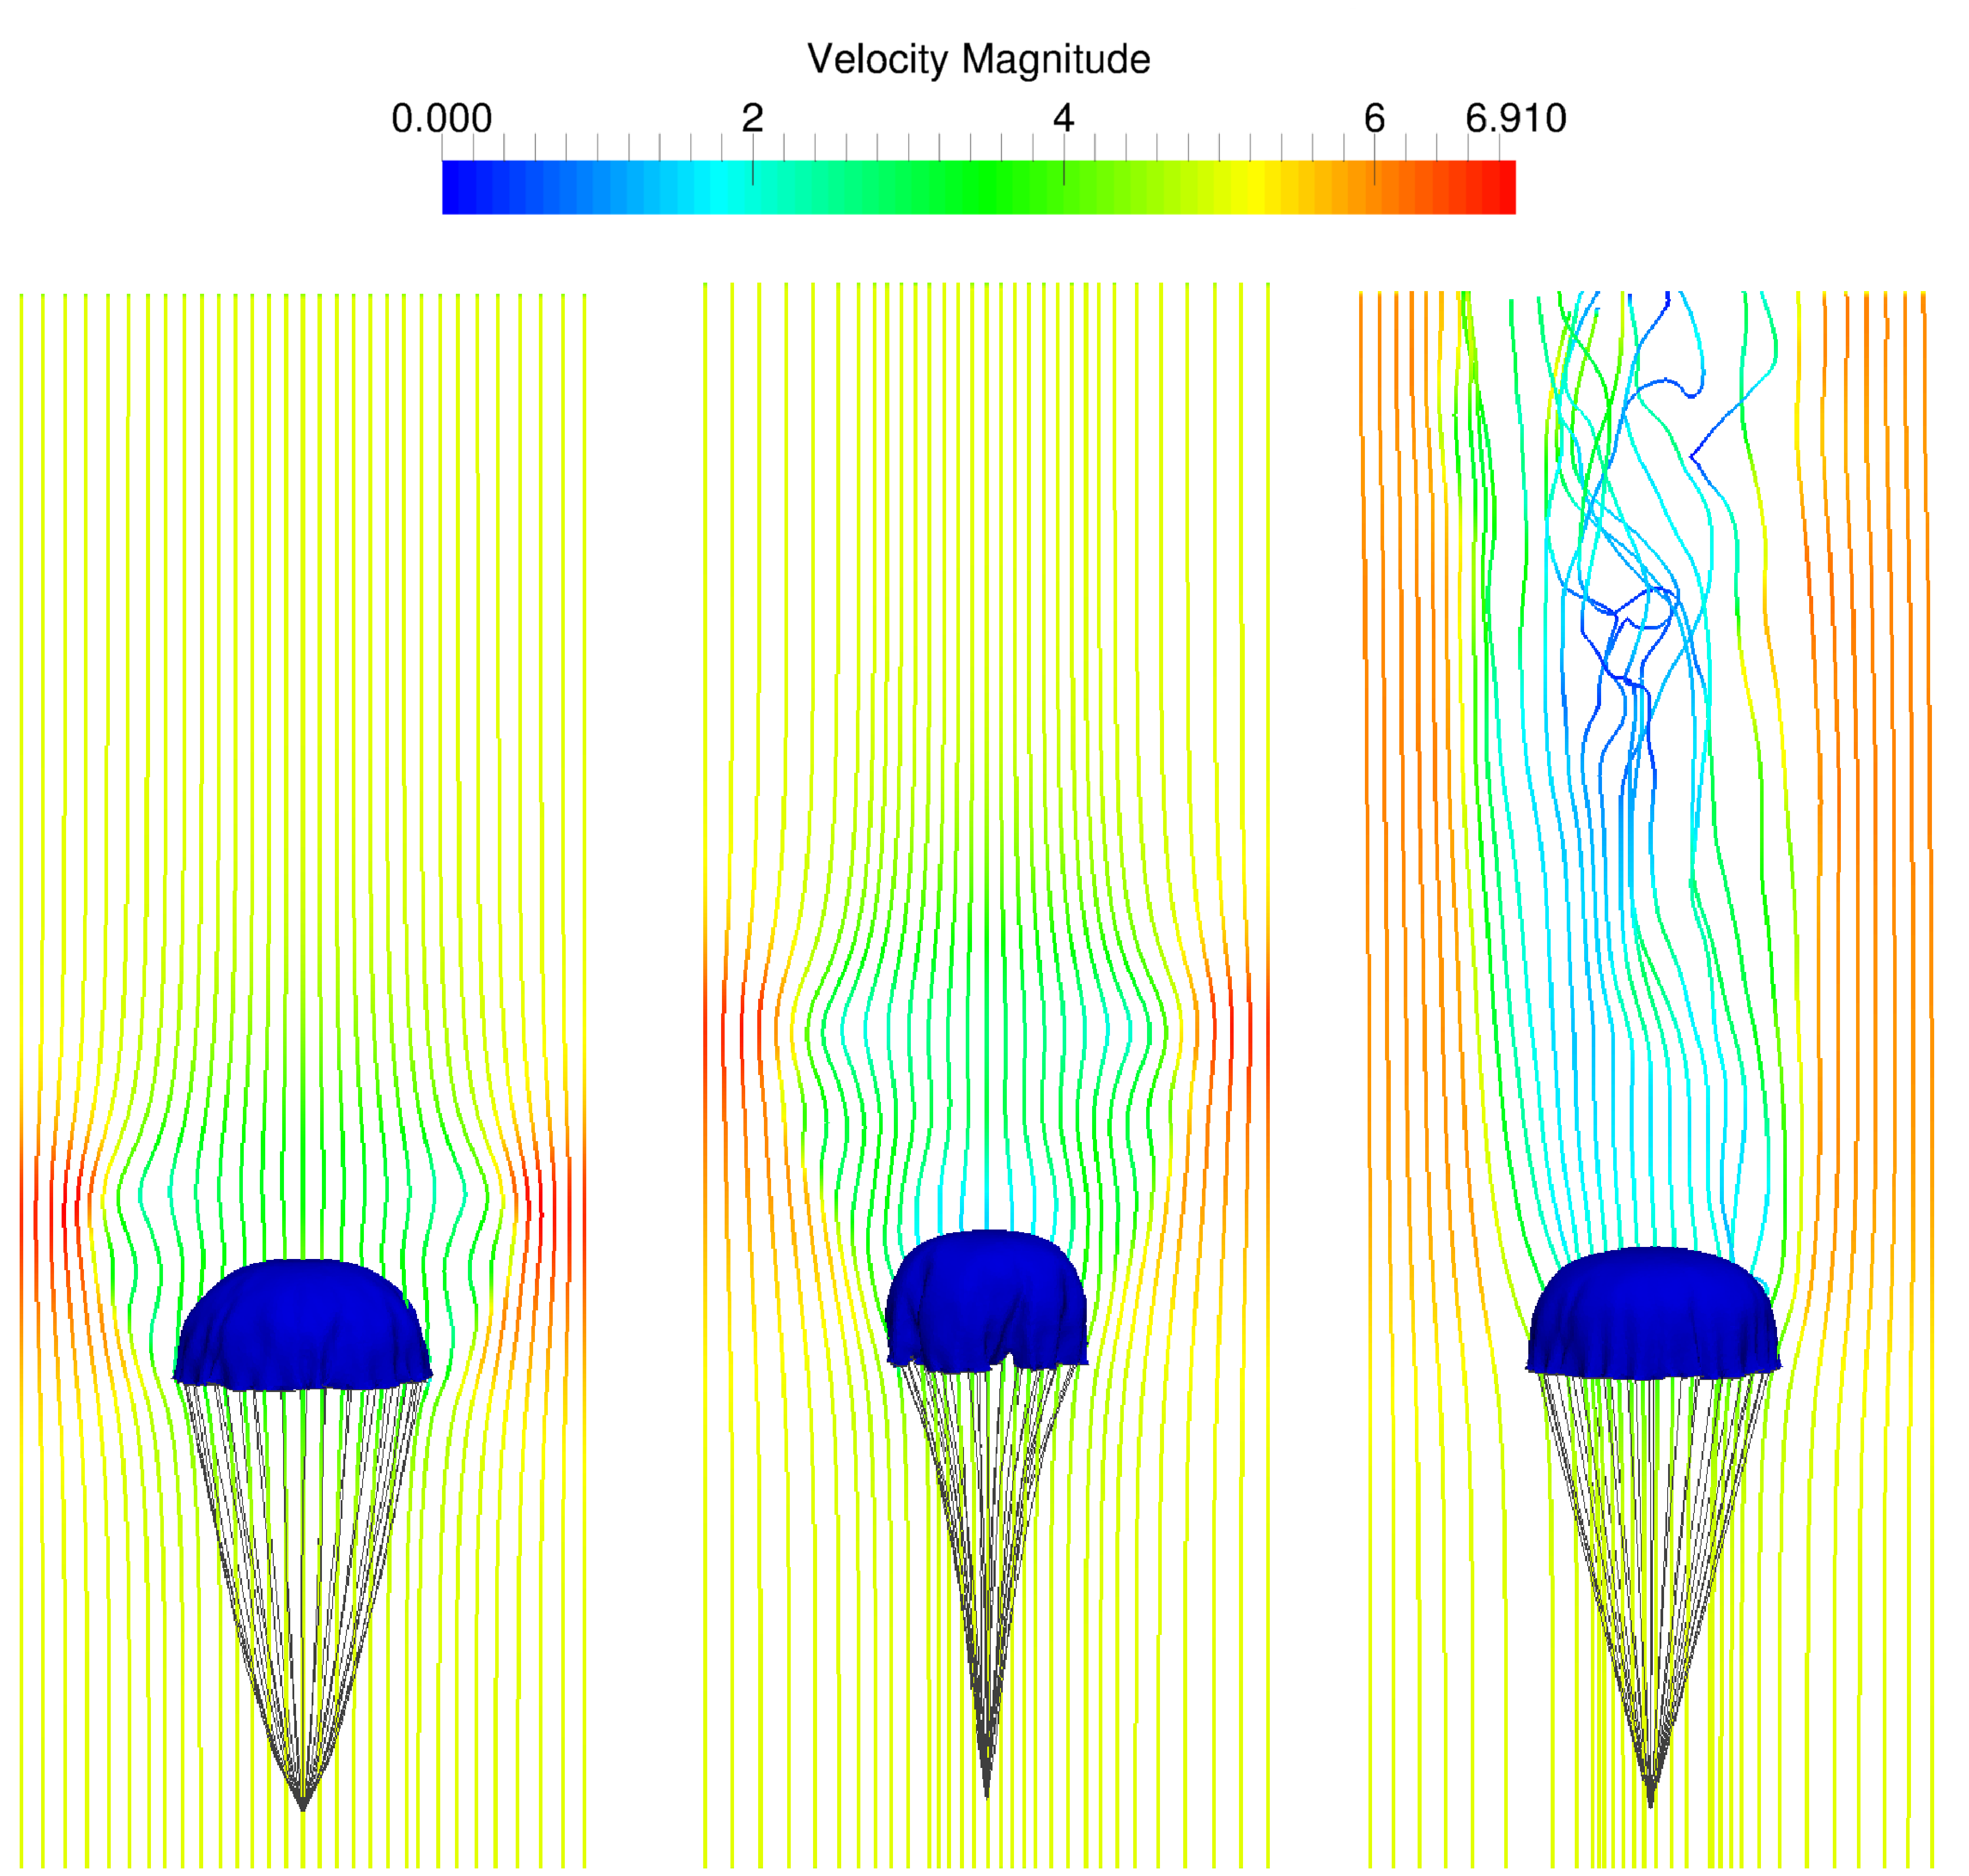
\includegraphics[width= 1.0\columnwidth]{Figures/drag_test} 
\caption{G11 cargo parachute in a numerical wind tunnel test
with the inlet velocity $5m/s$. The three plots from left to right are
the parachute shapes and velocity streamlines at 
the times $1.5s$, $2.5s$, and $15s$, respectively. The porosity 
coefficients in this case are set to be $\alpha = 6.7kgm^{-1}s^{-1}$, 
and $\beta = 3.1kgm^{-2}$. The oscillation of 
parachute canopy (parachute breathing) due to the elasticity of the parachute
string and the canopy is observed during the initial a few seconds. 
The streamlines are plotted with color 
to show the velocity magnitude.}
\label{fig:drag_test} \end{figure}

The drag force on the parachute is calculated by firstly integrating 
the pressure difference over all the surface elements (triangles) of the canopy 
and then projecting to the direction of the freestream velocity. After recording 
the drag force, the drag coefficient is calculated by the following formula: 
\begin{equation} 
C_d = \frac{F_d}{0.5\rho v^2_0A_0}
\label{eq:drag_coeff} 
\end{equation} 
where $\rho$ is the air density $= 1.2kg/m^3$, $v_0$ is the freestream velocity 
at the channel inlet and $A_0 = 78.5m^2$ is the area of parachute canopy at initial 
state. $F_d$ is the mean value of the drag force during the last $1s$ of the 
simulation. We observed that the drag coefficient increases at low descent velocities 
as displayed in \Table{table:drag_coeff}. This can be explained by the fact that the drag 
force (or the pressure drop) increases linearly at a very small velocity according to 
Ergun's equation, while the denominator has a quadratic growth.  

\begin{table}[H]
\centering
\begin{tabular}{cc}
\hline\hline
Inlet velocity ($m/s$) & Drag coefficients \\
\hline
$1.0$   & $1.89$ \\ 
$2.5$ & $1.31$ \\
$5.0$   & $0.92$ \\
$7.5$ & $0.63$ \\
$10.0$  & $0.49$\\
\hline
\end{tabular}
\caption{Drag measurements of the G11 parachute in wind tunnel tests
with varying inlet velocity and fixed the porosity coefficients 
$\alpha = 6.7kgm^{-1}s^{-1}$, $\beta = 3.1kgm^{-2}$.  
The drag coefficient decreases as the inlet velocity increases.}
\label{table:drag_coeff} \end{table}

To study the effects of the porosity on the parachute system,
we fix the inlet velocity at $3m/s$ while gradually increasing the
permeability of the parachute canopy. Although the porosity 
is not explicitly defined in our model, its relationship with the
parameters $\alpha$ and $\beta$ can be obtained
from the Ergun theory \cite{tutt2010development}:
\begin{equation}
\alpha = \frac{150\mu(1-\gamma)^2}{D^2\gamma^3}e, ~~~~
\beta  = \frac{1.75\rho(1-\gamma)}{D\gamma^3}e,
\end{equation}
where $\mu$ is the dynamic viscosity, $\rho$ is the density
of the air, $\gamma$ is the porosity of the parachute canopy,
$D$ is the characteristic length and $e$ is the thickness of the
porous surface. The porosity is defined 
as the fraction of the volume of voids over the total volume \cite{tutt2010development}.
Since the porosity is proportional to
$(\alpha/\beta^2)^{1/3}$, we can use the quantity  $(\alpha/\beta^2)^{1/3}$
instead of $\gamma$ to characterize the permeability of the
parachute canopy for our model. In fact, the parachute system is
affected by the porosity through in two ways. On one hand, the
porosity model will reduce the drag force on the parachute surface
by lowering the pressure difference. Since the viscous 
drag is ignored here, the pressure drag becomes the driving force affecting 
the shape and behaviors of the parachute.
On the other hand, the permeability
of parachute canopy could significantly affect the aerodynamic
field variables of the surrounding fluid such as pressure, flow velocity
and vorticity. These, in turn, will impact the stability of the
parachute system.

Another observation is that the parachute system would be more stable with
finite porosity than that of solely impermeable fabric.  This is shown by
comparing the drag force on the parachutes with and without fabric permeability
(see \Fig{fig:compare}).  

\begin{figure}[!htbp] \centering
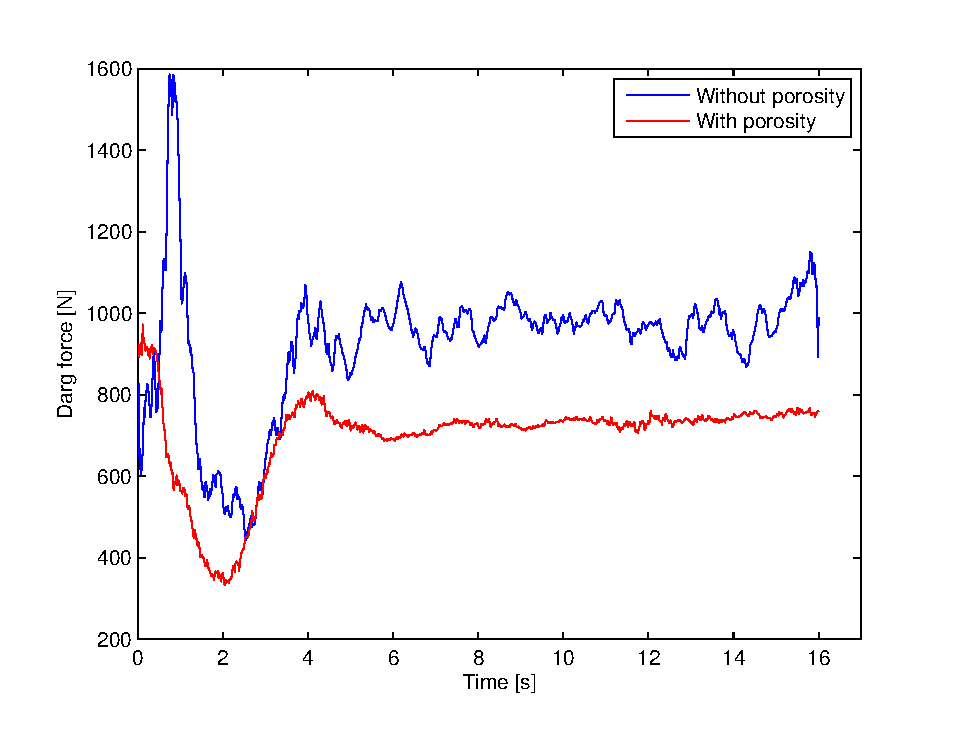
\includegraphics[width=1.0\columnwidth]{Figures/drag_compare} 
\caption{
Comparison of drag force for G11 parachute between the permeable (red) and 
impermeable (blue) canopies in the same simulation. The porosity coefficients 
are set to be $\alpha = 6.7kgm^{-1}s^{-1}$, $\beta = 3.1kgm^{-2}$. 
The increase of porosity leads to the reduction of drag force 
and the vorticity in the wake of the canopy, thus make the drag force
less oscillatory.} 
\label{fig:compare} 
\end{figure}

\subsection{Collision handling and folding algorithm}
In this section, the results of collision detection, collision handling, and 
folding algorithm are presented. Firstly, we have tested the performance of 
the collision handling algorithm. Several benchmark tests have been carried 
out: a round fabric falling on a rigid box; a round fabric falling on strings. 
These tests demonstrate the capability 
of our algorithm that can universally handle the interactions between fabric 
surface, rigid bodies and strings. \Fig{fig:collision_test} shows that the 
collision algorithm can produce visually plausible results and successfully 
eliminate all the intersections in the fabric. 
\begin{figure}[!htbp]
\includegraphics[width=0.45\columnwidth]{Figures/fabric-box.jpg}
\includegraphics[width=0.45\columnwidth]{Figures/fabric-string.jpg}
\caption{Benchmark test for collision detection and handling. Two cases are 
considered: interactions of fabric with rigid body (left) and elastic (right).
Note that the fabric's self-interactions are also handled well during the 
collision procedure.}
\label{fig:collision_test}
\end{figure}
In order to test the performance of 
the collision algorithm on a more complicated geometry, a simulation of a fabric
dropping from above of a rigid human model has been carried out. 
\Fig{fig:collision_test_human} displays three frames of the simulation and shows 
that the algorithm can well handle the collision between fabric and a non-trivial geometry.
\begin{figure}[!htbp]\centering
\includegraphics[width=0.3\columnwidth]{Figures/fabric-body-0.jpg}
\includegraphics[width=0.3\columnwidth]{Figures/fabric-body-1.jpg}
\includegraphics[width=0.3\columnwidth]{Figures/fabric-body-2.jpg}
\caption{Three movie frames in the simulation of collision between elastic fabric and rigid human model.}
\label{fig:collision_test_human}
\end{figure}

The folding algorithm is verified by close a round parachute canopy with $16$ creases. Here we name this folding pattern as ``close folding". Two groups of the folding angles are assigned corresponding to the mountain and valley crease alternatively. The final folding angle of the mountain crease is $-\pi$ and the folding angle of the valley crease is $3\pi/4$. The folding algorithm can automatically proceed and reach the desired state without any artificial controls. Three frames of the folding procedure are displayed in \Fig{fig:folding_para}. It can be seen that the canopy remains unstretched and the final state is perfectly symmetric. To explain the folding algorithm more clearly, the $16$ folding angles of the close folding are recorded and plotted in \Fig{fig:folding_angles}. The left panel is the behavior of the folding angles in the entire simulation and the right panel is a plot of the first $25$ steps. It is clear that the angles are moved randomly while gradually approach to the final state. This 
is because the optimization algorithm is based on a random search, and hence the folding angle can not be guaranteed to move uniformly. However, this behavior would not affect the eventually folded state, and in the meanwhile, the folding angles still strictly satisfy the necessary condition of the origami design. In conclusion, this folding algorithm provides a highly flexible and universal way to design various folding patterns. Only the folding angles and creases pattern are required as inputs while the intermediate folding process is completely automatic.
\begin{figure}[!htbp]\centering
\includegraphics[width=0.3\columnwidth]{Figures/fold-0.jpg}
\includegraphics[width=0.3\columnwidth]{Figures/fold-1.jpg}
\includegraphics[width=0.3\columnwidth]{Figures/fold-2.jpg}\\
\includegraphics[width=0.3\columnwidth]{Figures/fold-0.jpg}
\includegraphics[width=0.3\columnwidth]{Figures/fold-flat-1.jpg}
\includegraphics[width=0.3\columnwidth]{Figures/fold-flat-2.jpg}
\caption{Three movie frames of the parachute canopy shape in the folding process. The upper panel displays the close of a parachute canopy and the lower panel displays the flat fold.}
\label{fig:folding_para}
\end{figure}

\begin{figure}[!htbp]\centering
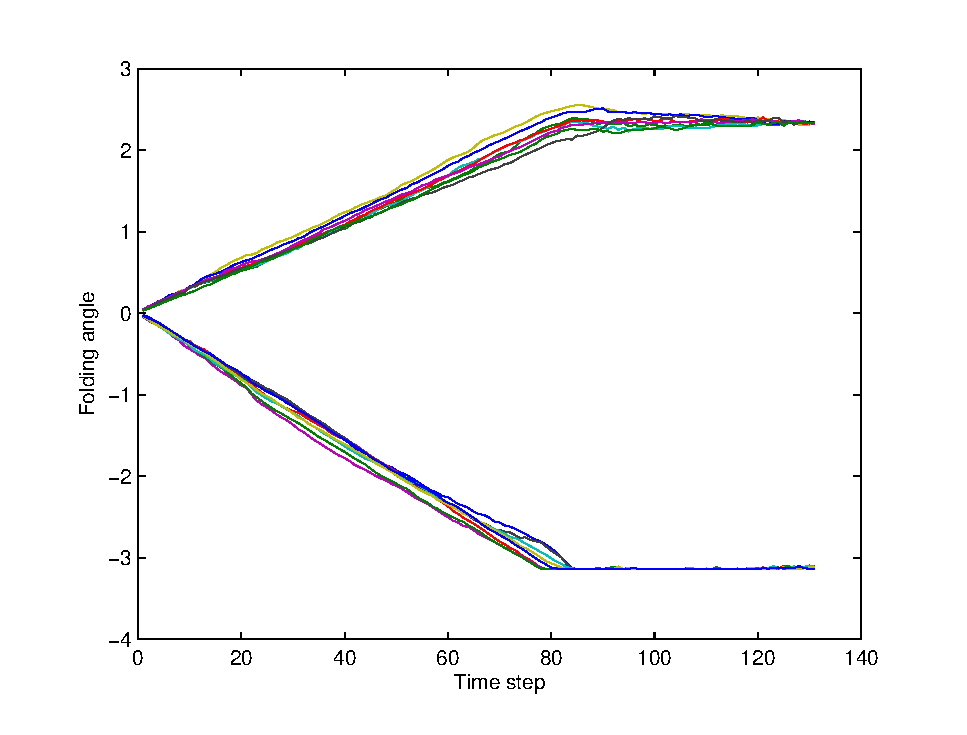
\includegraphics[width=0.45\columnwidth]{Figures/folding-angle}
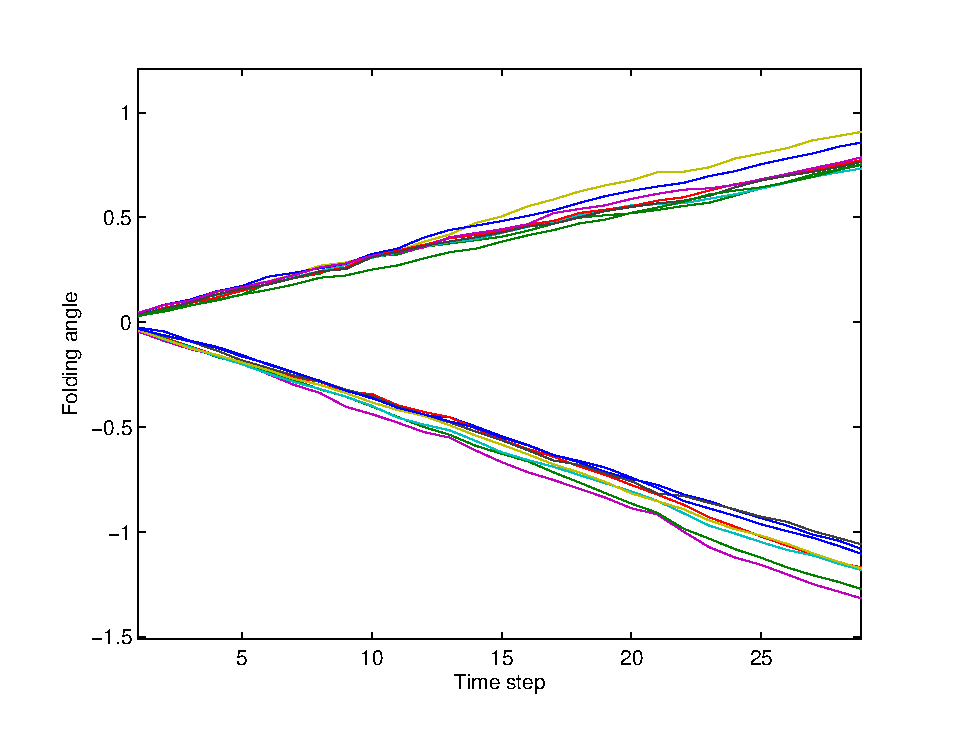
\includegraphics[width=0.45\columnwidth]{Figures/folding-angle-zoom}
\caption{Folding angles of the $16$ creases. Right panel shows the magnification of the irst $25$ steps.}
\label{fig:folding_angles}
\end{figure}

\section{Results for cloud entrainment and mixing}
\subsection{Experimental setup}
Three different initial configurations are used to investigate
the configuration impact. First, as in \cite{Andrejczuk2004}, the function of the water vapor mixing 
ratio $q_v(\vect{x}, t = 0)$ is defined according to the sign of the first component of the velocity 
field. This configuration is referred to as Case 1 and the water vapor mixing ratio is
given by

\begin{equation}
\mbox{case 1: } q_v(\mathbf{x},t=0) = 
\left\{\begin{array}{lr}
q_v^{max}, & u(\mathbf{x}) > 0\\
q_{v,e}, & u(\mathbf{x}) \le 0
\end{array}\right.\label{case1}
\end{equation}

In \cite{Kumar2012Cloud}, the author used a slab-like cloud configuration approximated by a continuous 
function with a rapid change at the cloud-clear air interface. We notice that this artificial function is 
used due to the shortcoming of the spectral method, which has the difficulty to handle the profile with discontinuities. Since a finite difference method is used here, we can simply replace this function with a discontinuous formula and refer it as Case 2:

\begin{equation}
\mbox{case 2: } q_v(x,t=0) = 
\left\{\begin{array}{lr}
q_v^{max}, & (L-d)/2 \le x < (L+d)/2\\
q_{v,e}, & \mbox{elsewhere}
\end{array}\right.\label{case2}
\end{equation}

where $q_v^{max}$ is maximum amplitude of $q_v$, which exceeds $q_{v,s}$ by
$2\%$, and $q_{v,e} = 0.03g/kg$ is the vapor mixing ratio of the clear air. $L$
is the length of computational domain, and $d = L/2$ is the width of the cloud
slab. The simulation is terminated when droplets completely evaporate or the
field becomes nearly uniform ($std<0.0002$).

Entrainment-mixing processes can also occur near cloud tops. To mimic the
cloud-top entrainment-mixing process, herein we add a new cloud configuration
by rotating Case 2 by $90$ degree, and name it Case 3.

\begin{equation}
\mbox{case 3: } q_v(z,t=0) = 
\left\{\begin{array}{lr}
q_v^{max}, & (L-d)/2 \le z < (L+d)/2\\
q_{v,e}, & \mbox{elsewhere}
\end{array}\right.\label{case3}
\end{equation}

The temperature field is initialized by imposing the neutral buoyancy condition \cite{Kumar2014Lagrangian}:
\begin{equation}
T(\vect{x},t = 0) = T_0 - 0.608T_0[q_v(\vect{x},t = 0) - q_{v,0}]
\end{equation}
where the reference values are defined by volume averages $T_0 = \langle
T(t=0)\rangle_V$ and $q_{v,0} = \langle q_v(t=0)\rangle_V$. This condition
implies that neither the vapor mixing ratio nor temperature would contribute to
the initial buoyancy. This procedure is only performed for the initial
temperature field and will completely follow \Eq{eq:Temp} afterwards.
\Fig{fig:slice_case123} illustrates the initial fields of water vapor mixing
ratio and temperature for the three cases.

\begin{figure}[!htbp]\centering
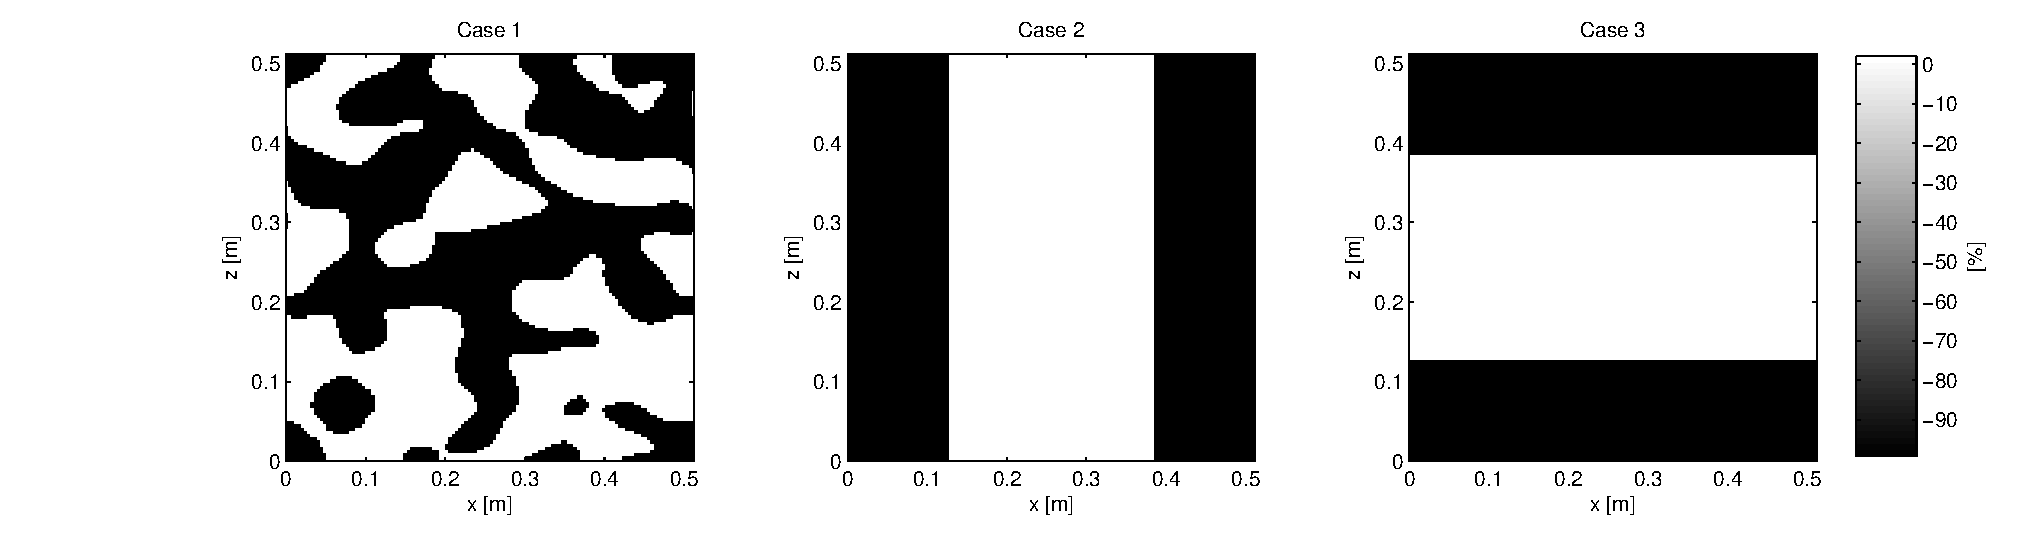
\includegraphics[width=0.95\textwidth]{Figures/supersat_case123}\\
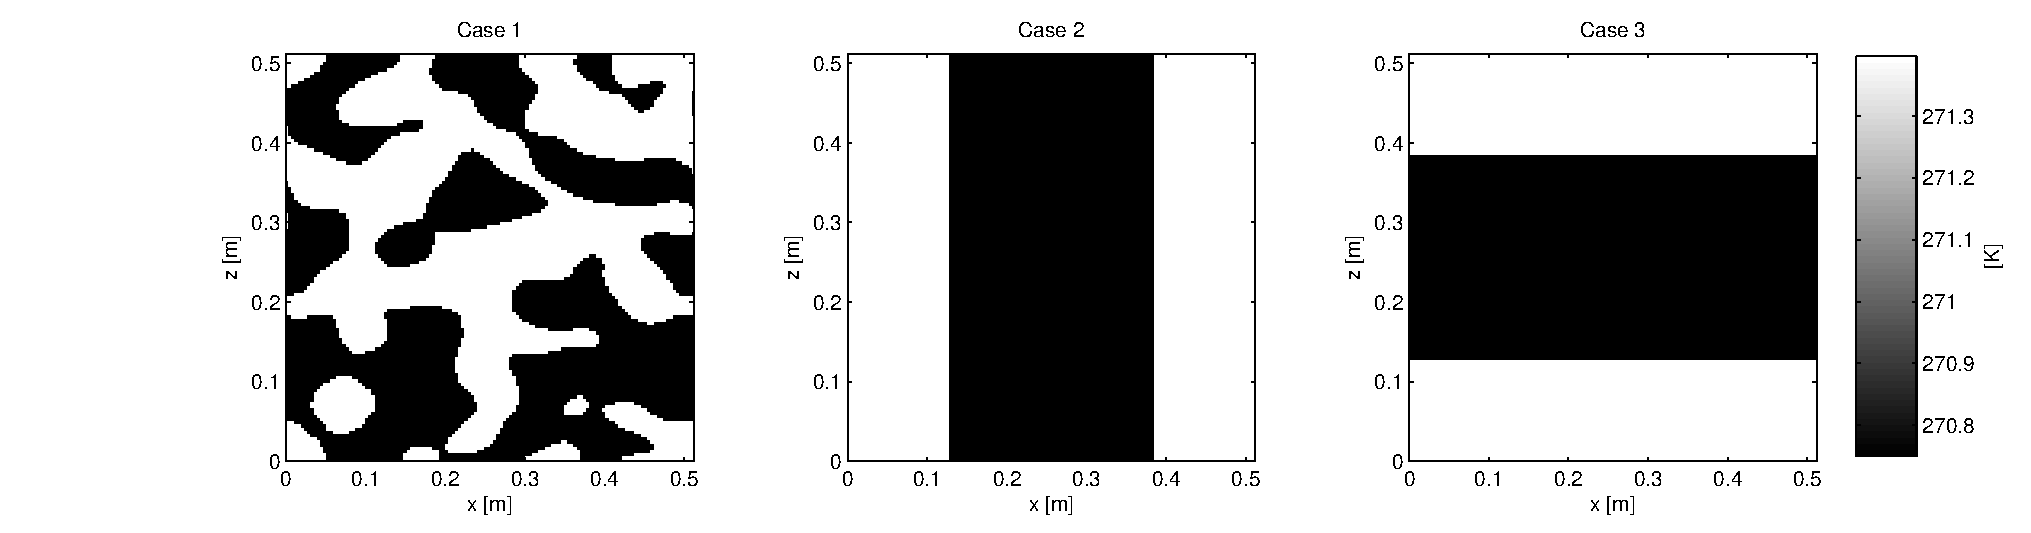
\includegraphics[width=0.95\textwidth]{Figures/temp_case123}
\caption{Cross sectional view of the initial supersaturation and temperature (K) field for different cases: case 1, 2, 3 from left to right. The cloudy part occupies about half of the computational domain.\label{fig:slice_case123}}
\end{figure}

At beginning, a total of $10^{7}$ droplets with the same radius of $15\mu m$
are uniformly placed in the cloudy area, so that the droplet number
concentration is about $153{cm}^{-3}$. Note that for the forced turbulence
scenario, the velocity field needs a few steps ($5$ seconds here) to relax to a
steady state. Therefore, the droplets are released to move and change their
sizes after this spin-up period. For the decaying
turbulence, the droplets are released at time $t = 0s$ since there is no needs
to seek for a steady state. A droplet with radius smaller than $1\mu m$ will be
immediately removed from the computational domain and will not contribute to
any statistical results.

For convenience, \Table{tb:parameters} summarizes the key quantities and initial conditions.
\begin{table}[!htbp]
\centering
\begin{adjustbox}{max width = \textwidth}
\begin{tabular}{l c c c c c}
\hline\hline
Quantity & Symbol & Value & Quantity & Symbol & Value\\
\hline
Grid points & $N$ & $256$ & Droplet radius & $R_{0}$ & $15\mu m$\\
Box length & $L$ & $0.512m$ & Environ supersat & $S_{e}$ & $-99\%$\\
Grid size & $a$ & $0.002m$ & Cloud supersat & $S_{c}$ & $2\%$\\
Viscosity & $\nu$ & $1.5\times10^{-5}m^{2}s^{-1}$ & Number density& $N_{c}$ & $153cm^{-3}$\\
Dissip rate& $\epsilon$ & $2.0\times10^{-3}m^{2}s^{-3}$ & Eddy turnover time & $\tau_{L}$ & $4.27s$\\
Dissip length& $\eta$ & $10^{-3}m$ & Evaporation time & $\tau_{evap}$ & $2.09s$\\
Dissip time& $\tau_{\eta}$ & $0.087s$ & Reaction time & $\tau_{react}$ & $4.52s$\\
\hline
\end{tabular}
\end{adjustbox}
\caption{Initial conditions}
\label{tb:parameters}
\end{table}

\subsection{Thermodynamics}
\Fig{fig:therm_dynam} compares the temporal evolution of the turbulent kinetic
energy (a), droplets number concentration (b), standard deviation and relative
dispersion of temperature (c,d) and the same for water vapor mixing ratio
(e,f).

In panel (a), the turbulent kinetic energy (TKE) of the forced cases F1, F2 and
F3 remains on average after a short relaxation at the initial time. However, it
is interesting to observe a transient growth in the decaying cases before
continuing to decay to zero. We interpret this growth as the results of
buoyancy effect, which is caused by the deviation of temperature and vapor
mixing ratio to the reference value according to \Eq{eq:source_term}. In
details, case D1 could be regarded as the intermediate stage of mixing process
in D2 or D3, therefore this deviation quickly disappear and show no growth in
the figure. As for D2, the mixing only happens at the interface between cloudy
and clear air, thus it takes much longer to damp the transient growth. The
mixing in case D3 is accelerated by sedimentation effect, making it a little
faster than D2.

The droplets number concentration for different cases are displayed in panel
(b). All cases have the same equilibrium state with a zero liquid water
content, i.e., all droplets eventually evaporate. The rate at which droplets
evaporate is higher for the forced turbulence than the decaying turbulence
except D1. In D1 all the droplets quickly be exposed to the same environment
and begin to evaporate, leading to its number concentration curve to be similar
as the forced cases.

Panel (c) and (d) show the standard deviation and relative dispersion of
temperature field. In spite of similar configuration with D2, case D3 has a
stronger growth in amplitude. We interpret this phenomenon as sedimentation
effect, indicating that the droplet movements are accelerated in the vertical
direction by gravity. Most of the droplets have a chance to enter into the
clear air and evaporate at an early stage. This evaporation process absorb
latent heat from the environment thus strongly making the temperature field
deviate from the mean value. However, this difference becomes smaller in the
forced turbulence since the motion of particles is predominantly controlled by
the external forcing, which are the same for F1, F2 and F3.

\Fig{fig:therm_dynam} (e) and (f) show the standard deviation and relative
dispersion of vapor mixing ratio, respectively. In these figures, we cannot
observe any transient growth as shown for temperature field. This result is
consistent with \cite{Kumar2014Lagrangian}. Notice that the vapor mixing ratio in the clear
air is much lower than in the cloudy air. The droplets entering into the clear
area will quickly turn into vapor while the droplets staying in the cloudy area
continue to condensate. This phase transition process reduce the difference of
vapor mixing ratio between clear air and cloudy air, thus the transient growth
of the deviation can hardly be observed.

\begin{figure}[!htbp]\centering 
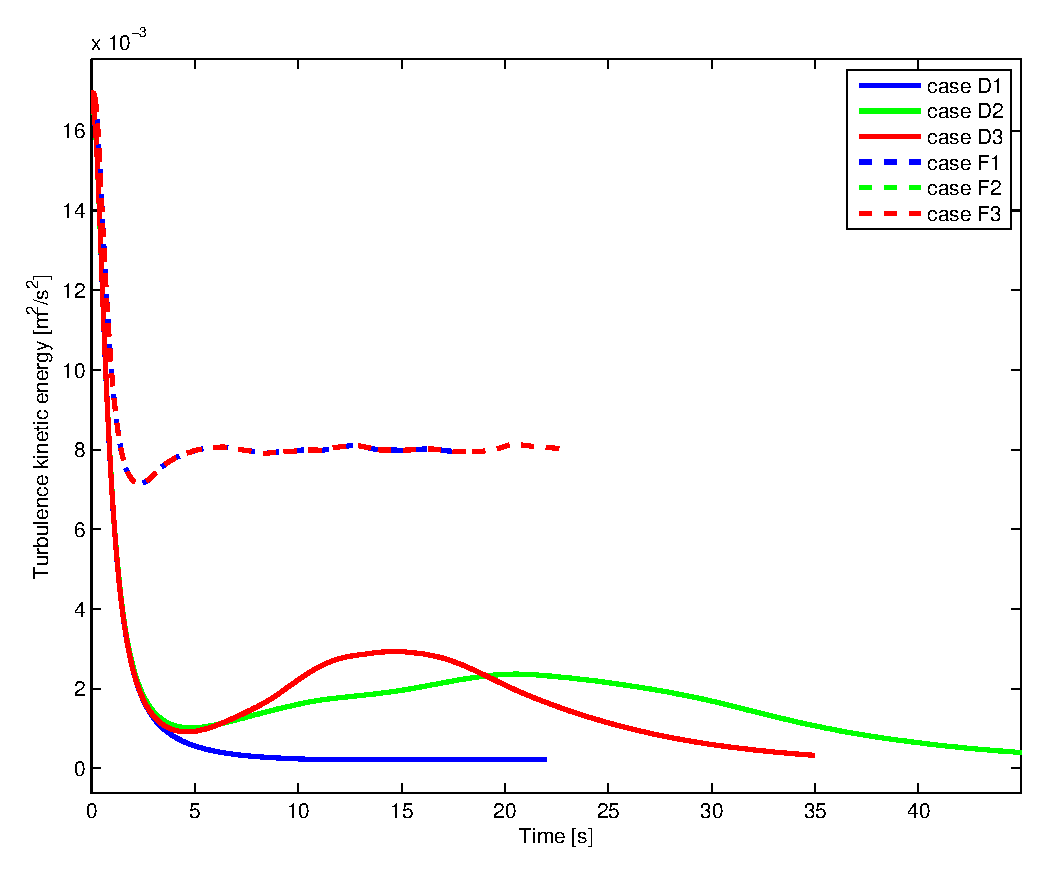
\includegraphics[width=0.4\textwidth]{Figures/tke}
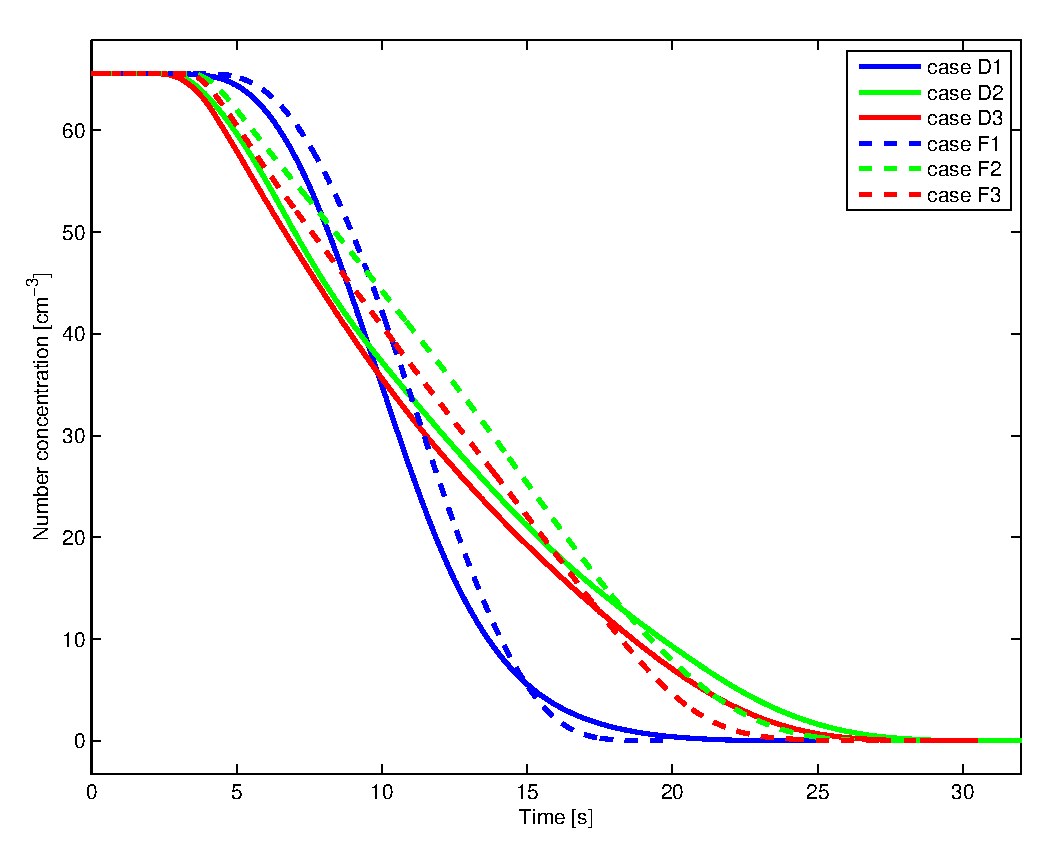
\includegraphics[width=0.4\textwidth]{Figures/num_con}\\
\includegraphics[width=0.4\textwidth]{Figures/temp_std}
\includegraphics[width=0.4\textwidth]{Figures/temp_dsp}\\
\includegraphics[width=0.4\textwidth]{Figures/vapor_std}
\includegraphics[width=0.4\textwidth]{Figures/vapor_dsp}
\caption{From thermodynamics variables as a function of time. From left to right, 
up to bottom, are turbulence kinetic energy (a), droplets number 
concentration (b), standard deviation (c), relative dispersion (d) of 
temperature field and the same for the vapor mixing ratio (e,f).}\label{fig:therm_dynam} 
\end{figure}

\subsection{Microphysics}
The droplet size distributions for case 1, 2 ,3 in both decaying and forced
turbulence are displayed in \Fig{fig:rad_distri}. At the initial stage, some
droplets enter into the clear air and expand their size distribution. As mixing
going on, since the environment is unsaturated and homogeneous, the
distribution gradually shift to small sizes until all droplets completely
evaporate or the background environment becomes saturated.  An important
observation is that case D1, D2 and D3 are quite different in size distribution. 
However, by adding the external force, these
difference almost disappear. This demonstrates that the role of buoyancy effect
is overwhelmed by the external forcing and the differences in the decaying
cases are caused by the buoyancy term in \Eq{eq:source_term}. In specific, the
buoyancy plays as a source of kinetic energy, so as to influence the motion of
the fluid field.  

\begin{figure}[H]\centering
\subcaptionbox{}{\includegraphics[width=0.45\textwidth]{Figures/pdf_radius_d1}}
\subcaptionbox{}{\includegraphics[width=0.45\textwidth]{Figures/pdf_radius_f1}}
\end{figure}

\begin{figure}[H]\ContinuedFloat\centering
\subcaptionbox{}{\includegraphics[width=0.45\textwidth]{Figures/pdf_radius_d2}}
\subcaptionbox{}{\includegraphics[width=0.45\textwidth]{Figures/pdf_radius_f2}}
\end{figure}

\begin{figure}[H]\ContinuedFloat\centering
\subcaptionbox{}{\includegraphics[width=0.45\textwidth]{Figures/pdf_radius_d3}}
\subcaptionbox{}{\includegraphics[width=0.45\textwidth]{Figures/pdf_radius_f3}}
\caption{Evolution of radius distribution for decaying turbulence (left column)
and forced turbulence (right column). From up to bottom are case 1, case 2 and
case 3 respectively.}\label{fig:rad_distri} \end{figure}

The distribution of supersaturation in \Fig{fig:supersat_distri} also clearly
reflects the mixing process. In the initial period, most of the droplets stay
in the cloud filaments, and thus has narrow probability density distribution
(PDF). After some droplets entering into the clear air, the spectrum
immediately expands with low probability density. This stage could be observed
in D2 and D3, but extremely short for the rest cases. As mixing proceeds, the
environment becomes much more homogeneous, that is most droplets stay in a
similar environment. Finally, the environment becomes well-mixed, droplets
completely evaporate and all the cases reach the same state. 

In conclusion, the shape of the cloud
filament has no influence on the final state after the mixing but will affect
the intermediate process. The shape also has little impact on the mixing
process for forced turbulence, while can not be completely ignored in the
decaying cases. The results suggest that the initial shape of cloud filaments
should be considered as an important factor when studying mixing scenario
without external forcing.

\begin{figure}[!htbp]\centering
\includegraphics[width=0.48\textwidth]{Figures/pdf_supersat_d1}
\includegraphics[width=0.48\textwidth]{Figures/pdf_supersat_f1}\\
\includegraphics[width=0.48\textwidth]{Figures/pdf_supersat_d2}
\includegraphics[width=0.48\textwidth]{Figures/pdf_supersat_f2}\\
\includegraphics[width=0.48\textwidth]{Figures/pdf_supersat_d3}
\includegraphics[width=0.48\textwidth]{Figures/pdf_supersat_f3}
\caption{Evolution of supersaturation distribution for decaying turbulence
(left column) and forced turbulence (right column). From up to bottom are case
1, case 2 and case 3 respectively.}\label{fig:supersat_distri} \end{figure}

\subsection{Entrainment-mixing processes}
Following the conceptual picture contributed by \cite{Krueger1997Modeling,Grabowski1993Cumulus, Burnet2007Observational}, 
the entrainment mixing process can be described by the following sequence of states.  
Firstly, driven by the convective circulation, a portion of the cloudy air is replaced 
by the environmental air. The cloud droplets are diluted and the mean radius remains 
unchanged. Then the cloud droplets may evaporate or grow in process of mixing, and the details 
depends on the specific mixing mechanisms. In the homogeneous mixing, the phase relaxation of cloud water droplets is 
slow compared to the mixing time, and hence the droplets stay in a well-mixed and 
homogeneous environment. Before any droplets completely evaporate, the number concentration 
of the cloud droplets remains unchanged. In the opposite scenario, inhomogeneous 
mixing, where evaporation proceeds much faster than the turbulence evolves, 
the cloud droplets are exposure to different humidity. Therefore, the number concentration 
decreases due to the complete evaporation of some droplets, while the mean radius
keeps the same. In reality, both scenarios can coexist in a turbulent cloud since 
a whole spectrum of fluid timescale is present \cite{Lehmann2009} and most mixing process 
fall between the two extremes.

The above mixing process can be characterized by the Damk{\"o}hler number, the ratio of 
a fluid timescale to a thermodynamic timescale associated with the evaporation:

\begin{equation}
Da=\frac{\tau_{mix}}{\tau_{react}}\label{eq:DaNumber}
\end{equation}
where the turbulence mixing time scale can be estimated as $\tau_{mix} = (\lambda^2/\epsilon)^{1/3}$; 
the length scale $\lambda$ is represented by the mean Taylor microscale \cite{Andrejczuk2009} for the cloud water, $\lambda = 
(\lambda_1+\lambda_2+\lambda_3)/3$, $\lambda_i = \langle q_c^2\rangle^{1/2}/\langle(\partial q_c/
\partial x_i)^2\rangle^{1/2}$, and the dissipation rate is estimated with $\epsilon = 2\nu\langle(\nabla
\times \mathbf{u})^2\rangle$. The droplet evaporation time scale $\tau_{react}$ will be introduced later. In general, $Da\ll1$ corresponds to the homogeneous mixing while $Da\gg1$ is
the inhomogeneous one. Ambient clouds often have $Da$ between these two limits.

Another dynamic measure of the occurrence probability of homogeneous or inhomogeneous 
mixing process is the transition scale number \cite{Lu2011} defined as the ratio of 
the transition length $l^{*}$ and the Kolmogorov length scale $\eta$:
\begin{equation}
N_{L}=\frac{l^{*}}{\eta}\label{eq:NL}
\end{equation}
 
where $l^{*}$ is defined as the length, at which mixing transits from inhomogeneous 
to homogeneous \cite{Lehmann2009}:
\[
l^{*}=\epsilon^{1/2}\tau_{react}^{3/2}
\]
and 
\[
\eta = (\frac{\nu^3}{\epsilon})^{1/3}, 
\]
$\nu$ is the kinematic viscosity and $\epsilon$ is the dissipation rate.

The reaction time scale can be estimated in two ways. 
In \cite{Andrejczuk2009, Burnet2007Observational}, it is defined as the time that a droplet needs 
to complete the evaporation:
\begin{equation}
\tau_{evap} = R_v(\frac{dR_v}{dt})^{-1} = \frac{R_v^2}{-KS_e}
\end{equation}
where $R_v$ is the mean volume radius of a group of droplets; $K$ is the constant in the 
droplet diffusional growth equation, and $S_e$ is the supersaturation of the dry air. 
This definition assumes that the environmental dry air is always 
sufficient and never becomes saturated during the evaporation. Therefore, this definition 
can only deal with an unsaturated environmental air where $S_e$ is negative.

In \cite{Lehmann2009, Lu2013}, $\tau_{react}$ is defined as the time when droplets have completely 
evaporated or relatively humidity has reached $99.5\%$ whichever is first satisfied. It is calculated 
by solving the following coupled ordinary differential equation for the mean volume radius and mean supersaturation:

\begin{equation}
\frac{dR_{v}}{dt}=K\frac{S}{R_{v}}\label{eq:DiffR}
\end{equation}

\begin{equation}
\frac{dS}{dt}=-BR_{v}S\label{eq:DiffSuper}
\end{equation}
where $B$ is a function of pressure and temperature:
\begin{equation}
B = 
\frac{4\pi N\rho_L[\frac{R_dT}{\varepsilon e_s(T)} + \frac{\varepsilon L^2_h}{pTc_p}]} 
{(\frac{L_h}{R_vT}-1)\frac{L_h\rho_L}{KT} + \frac{\rho_L R_v T}{De_s(T)}}
\end{equation}

where $L_h$ is latent heat, $R_v$ is individual gas constant for water vapor,
$T$ is air temperature, $\rho_L$ is density of liquid water, $K$ is coefficient
of thermal conductivity of air, $D$ is coefficient of diffusion of water vapor
in air, $e_s(T)$ is saturation vapor pressure over a plane water surface at
temperature $T$, $N$ is number concentration of droplets, $R_d$ is individual
gas constant for dry air, $\varepsilon = R'/R_v$, $p$ is air pressure, and
$c_p$ is specific heat with pressure held constant \cite{Lu2011}.
This definition considers the interactions between liquid water and vapor water, 
and hence its value is expected to be smaller than the previous definition. 

To characterize the microphysical properties of the mixing, the $R_v^3-N_d$ 
diagram was introduced in \cite{Burnet2007Observational} and has been widely applied to study the
entrainment-mixing process. To define the number 
density and mean volume radius, it is necessary to define a sample box. Hence 
the computational domain is divided into $64$ equal-sized sample boxes. We keep 
tracking the volume mean radius and number concentration at each time step in 
each sample box. The mixing diagrams for different cases are displayed in 
\Fig{fig:mixing_diagram}. Since homogeneous mixing corresponds to the horizontal 
line in the $R_v^3-N$ diagram, whereas the vertical line implies extremely inhomogeneous 
mixing \cite{Andrejczuk2009}, the homogeneous mixing degree can be quantified by the instantaneous slope 
of the trajectories in the diagram, and is calculated using centered differencing 
in time:
\begin{equation}
\psi_0 = \frac{N_{j+1}/N_a - N_{j-1}/N_a}{R_{j+1}^3/R_a^3 - R_{j-1}^3/R_a^3}
\label{phi0}
\end{equation}

More measures of homogeneous mixing degree have been introduced in \cite{Lu2011, Lu2014}. 
These definitions are based on the mixing of adiabatic cloudy air and clear air. 
However, in this paper, the instantaneous homogeneous mixing degree is calculated from 
two adjacent states in time $t_j$ and $t_{j-1}$, and hence the cloudy air may have been 
diluted and the environmental air may contains droplets. This implies that the original 
assumption does not hold and some modifications are required. The four modified definitions 
of the homogeneous mixing degree are listed below according to \cite{Lu2011, Lu2014}.

\begin{equation}
\psi_1 = \frac{\tan^{-1}(\frac{R_{j}^3/R_{j-1}^3 - 1}{N_j/N_{j-1} - N_h/N_{j-1}})}{\pi/2}
\label{phi1}
\end{equation}

\begin{equation}
\psi_2 = 0.5(\frac{N_j-N_{i}}{N_h-N_i} + \frac{R_j^3-R_{j-1}^3}{R_h^3 - R_{j-1}^3})
\label{phi2}
\end{equation}

\begin{equation}
\psi_3 = \frac{\ln R_j^3 - \ln R_{j-1}^3}{\ln R_{vh}^3 - \ln R_{j-1}^3}
\label{phi3}
\end{equation}

\begin{equation}
\psi_4 = \frac{1 - R_{j}^3/R_{j-1}^3}{1 - LWC_{j}N_{j-1}/(N_h LWC_{j-1})}
\label{phi4}
\end{equation}

where all the variables are calculated from a sample box; $R$ is the mean volume radius; $N$ is the number density; $LWC$ is the liquid water content; the index $j$ means the value is calculated from the $j$-th dataset at time $t_j$. The indicies $i$ and $h$ indicate that the values are calculated based on the assumption of inhomogeneous and homogeneous mixing. The variables $R_h$, $N_i$ and $N_h$ are calculated as below:
\[
R_h^3 = \frac{N_jR_j^3}{N_h},
\]

\[
N_i = \frac{R_j^3}{R_{j-1}^3}N_j.
\]

\[
N_h = \chi N_j + (1 - \chi) Ne_j
\]

The mixing fraction $\chi$ is computed according to the mass conservation of total water between state $j$ and $j-1$:
\begin{equation}
\chi(q^{j-1}_{vc} + q^{j-1}_{lc}) + (1-\chi)(q^{j-1}_{ve} + q^{j-1}_{le}) = q^{j}_{lc} + q^{j}_{vc}
\end{equation}
where $q$ is the water mixing ratio; indicies $c$ and $e$ stand for the mean 
value of a sample box and its environmental air; $l$ and $v$ stand for the liquid 
water and vapor water. The environmental air is defined as the air in $4$ 
grids extended from the original sample box; $j$ indicates the state of the $j$-th dataset 
collected at time $t_j$.

Before proceeding to the discussion of the the result, we need to show that the 
four definitions of homogeneous mixing degree are reasonable and can cover the 
two extreme cases: $1$ for homogeneous mixing and $0$ for inhomogeneous mixing. 
When a mixing process is extreme inhomogeneous, the volume mean radius equals 
to the value in previous time step $R_{j-1}$, and hence the corresponding number 
concentration is $N_i = R^3_{j}N_j/R^3_{j-1}$. Given $R_j = R_{j-1}$ and 
$N_j = N_i$, it is straightforward to have $\psi_1$, $\psi_2$, $\psi_3$ and $\psi_4$
all equal to zero. When a mixing process is homogeneous, the number concentration can be 
approximated as a linear combination of the cloudy air and the environmental air, that is $N_h = 
\chi N_{j-1} + (1-\chi)N_{e,j-1}$. Assuming the liquid water content at time $t_j$ is a constant, 
the homogeneous mean  volume radius is calculated as $R_h^3 = N_jR_j^3/N_h$. A homogeneous 
mixing implies that $N_j$ is close to $N_h$ and $R_j$ approaches to $R_h$, thus it is 
easy to derive that $\psi_1$, $\psi_2$ and $\psi_3$ equal to $1$. 
As for $\psi_4$ in the homogeneous mixing, conditions $N_j = N_h$, 
and $R_j = R_{j-1}$ yield
\[
\frac{N_{j-1}LWC_j}{N_hLWC_{j-1}} = \frac{N_{j-1}R_j^3N_h}{N_hR_{j-1}^3N_{j-1}}
= \frac{R_j^3}{R_{j-1}^3},
\]
and hence $\psi_4$ also equals to one. \Fig{rn_diagram} illustrates the meaning of these 
intermediate variables.

\begin{figure}[!htbp]
\includegraphics[width=\textwidth]{Figures/mix_dia}
\caption{Illustration of $R_h^3$, $N_i$ and $N_h$ in a mixing diagram. The liquid water 
content is assumed to decrease to $0.2$ of the same from last step.\label{rn_diagram}}
\end{figure}
 
 
\Fig{fig:mixing_diagram} shows the mixing in the sample boxes. The 
circles represent the values sampled in the each sample box at each time step; 
the mixing trajectory from the whole DNS domain is plotted using solid 
lines with arrows indicating the direction of temporal evolution; the homogeneous mixing line and 
inhomogeneous mixing line are plotted in the diagram as references. 
In the top panel, the mixing diagram of D1 and F1 do not start from the $(1,1)$ 
point since the initial droplets in a sample box have already been diluted and 
their number concentration are much less than the adiabatic value. The droplets number concentration remains nearly unchanged until some droplets completely evaporate. 
As claimed in \cite{Andrejczuk2004}, this configuration excludes the dilution process and 
can only be used to simulate the final stage of the entrainment and mixing process. 
The difference between forced turbulence and decaying turbulence is not 
obvious, except a wider range of variability in the shape of the mixing 
trajectories for the decaying turbulence D1, since the forced turbulence 
will foster the mixing procedure, resulting in similar states in different 
sample boxes.

In the middle panel, the mixing diagram shows the mixing curves for case D2 and
F2. These cases have the same configurations with \cite{Kumar2014Lagrangian}. However, a
sharp initial profile of vapor mixing ratio was used in our simulation. This
results in an unsaturated vapor mixing ratio at final state, leading to
completely evaporation of the droplets. The phenomenon of inhomogeneous offset
described by \cite{Kumar2014Lagrangian} could also be observed in the figures: the mixing
trajectories tend to shift to smaller values of $N_d/N_{d,a}$. This
inhomogeneous offset is almost due to the initial dilution process, in which
the droplets number concentration in the sample boxes is diluted while the
droplets mean radius in the sample box doesn't change too much. As mixing
proceeds, the turbulent time scale in the decaying case continues to increase
while the time scale for the forced turbulence remains unchanged. Therefore,
the inhomogeneous mixing is more likely to happen in case D2, leading to a
strong deviation from the homogeneous mixing line.

A similar conclusion can be obtained in the bottom panel for case D3 and F3.
However, it is interesting to observe two groups in the mixing trajectories. We
interpret this divergence by considering the following facts. According to our
way of selecting sample boxes, the cloud slab will be divided into two groups:
the upper layer and the lower layer. On one hand, due to the
sedimentation effect, a part of the droplets will escape from the upper layer
and enter into the lower layer, thus making the number concentration of upper
level sample boxes decreased and their volume mean radius unchanged. On the
other hand, the evaporating droplets below the lower layer may reentering into
the lower sample boxes by the turbulent mixing, leading to reduced volume mean
radius and slowly decreasing number concentration.

\begin{figure}[!htbp]\centering
\includegraphics[width=0.4\textwidth]{Figures/mixing_cased1}
\includegraphics[width=0.4\textwidth]{Figures/mixing_casef1}\\
\includegraphics[width=0.4\textwidth]{Figures/mixing_cased2}
\includegraphics[width=0.4\textwidth]{Figures/mixing_casef2}\\
\includegraphics[width=0.4\textwidth]{Figures/mixing_cased3}
\includegraphics[width=0.4\textwidth]{Figures/mixing_casef3}
\caption{Mixing diagram for case D1, D2, D3, F1, F2 and F3. Mean cubic radius
and mixing fraction have been calculated in 64 equal-sized samples boxes. The
circle represent the time trajectories of $R_v^3/R_{v,0}^3$ and $N_d/N_{d,a}$
in different sample boxes and the triangles represent the same in the entire
domain. Color indicates the time for each record. Only the boxes with non-zero
particles at the initial time are considered.}
\label{fig:mixing_diagram}
\end{figure}

The transition scale number , Damk\"{o}hler number and the 
microphysical measures of homogeneous mixing degree are expected 
to be correlated since they are measures quantifying the probability of 
the homogeneous mixing process from different perspective. These relationship are examined using 
the numerical data produced from case $1$, $2$, $3$ in the decaying and forced turbulence. First, 
the slope \ref{phi0} is plotted with the Damk\"{o}hler number and transition scale number in \Fig{fig:slope_da_nl}. The left figure shows that the Damk\"{o}hler number has a positive relationship with the reciprocal of the slope. This duplicates the results in \cite{Andrejczuk2009} and is consistent with the heuristic argument relating homogeneity of mixing to the time scale ratio. We also compare the results using transition scale number and Damk\"{o}hler number as the dynamical measures in the right figure. It yields that the transition scale number has a wider range of values but gives consistent conclusion with Damk\"{o}ler number.

\begin{figure}[!htbp]\centering
\includegraphics[width=0.49\textwidth]{Figures/slope_da}
\includegraphics[width=0.49\textwidth]{Figures/slope_da_nl}
\caption{The left figure displays the scatter plot of the slope in the $R-N$ diagram as a function 
of Damk\"{o}hler number and transition scale number. The comparison between using Damk\"{o}hler 
number and transition scale number is shown in the right figure.}
\label{fig:slope_da_nl}
\end{figure}

The scatterplot of the mixing degree as a function of the transition scale number is shown in \Fig{fig:mix_degree_nl} with color indicating the normalized simulation time. The fitting curves have a close slope for different cases, and a tight relationship can be clearly observed in the critical range of the slopes, and therefore one can suggest a simple parameterization.
\begin{figure}[!htbp]\centering
\includegraphics[width=0.49\textwidth]{Figures/phi1_NL}
\includegraphics[width=0.49\textwidth]{Figures/phi2_NL}\\
\includegraphics[width=0.49\textwidth]{Figures/phi3_NL}
\includegraphics[width=0.49\textwidth]{Figures/phi4_NL}
\caption{Scatter plot of the homogeneous mixing degree vs the transition scale number. All the cases are shown in one figure. From left to right, up to bottom are $\psi_1$, $\psi_2$, $\psi_3$ and $\psi_4$.\label{fig:mix_degree_nl}}
\end{figure}

The quantities mentioned at the beginning of this section can be used as good
predictors of the mixing scenario. As shown in \Table{tb:parameters}, the eddy
turnover time $\tau_L = 4.27s$, evaporation time scale $\tau_{evap} = 2.09s$
and reaction time scale $\tau_{react} = 4.52s$. Defining a Damkohler number
based on $\tau_{evap}$ gives $Da_{L,evap} = 2.04$, which is significantly
greater than unity and seems to favor a strong inhomogeneous mixing in the
inertial range. However, during mixing, the evaporation of droplets gradually
saturate surrounding vapor and therefore the chemical reaction will spend
longer time to complete. This implies that the assumption of constant
supersaturation for the $\tau_{evap}$ is not strictly correct.  As opposed to
$\tau_{evap}$, the definition of $\tau_{react}$ based on \Eq{eq:DiffR} and
\Eq{eq:DiffSuper} considers the interactions between radius $R$ and
supersaturation $S$ and therefore should be more suitable to predict the
thermodynamic time scale. Defining the Damkohler number based on $\tau_{react}$
results in $Da_{L,react} = 0.94$, slightly lower than unity and hence yields an
intermediate state between the homogeneous and inhomogeneous mixing. In fact,
the transition length scale is equal to $l^{*} = 0.426m$, defining the length
scale within the inertial range at which $Da = 1$. This $l^*$ is somewhat
smaller than the domain size $0.512m$ but $400$ times greater than the
Kolmogorov length scale. As the turbulence eddies evolve from the energy
containing length $L_x$, through $l^*$, and down to the smallest length scale
$\eta$, the mixing scenario quickly expands from inhomogeneous to homogeneous
mixing. The side length of the sample boxes $0.512m/4 = 0.128 m$ is
significantly smaller than $l^* = 0.426m$, thus an extreme homogeneous mixing
is most possible to be observed. However, from \Fig{fig:mixing_diagram}, the
relationship between the mixing trajectory and mixing scenario is not obvious.
The mixing trajectories do not have to follow the homogeneous mixing line
although the mixing scenario is expected to be homogeneous. Moreover, the
behaviors of the mixing trajectories for different cases differ from each other
even if they have the same liquid water content and initial turbulence
settings. In conclusion, the behaviors of the mixing trajectories are not only
determined by the relative time scale or Damkohler number but also by the
distribution of the cloud water content.

\subsection{Preferential concentration}
The clustering of inertial particles has been extensively studied via both
experiments and numerical simulations \cite{Sundaram1997Collision, Reade2000Effect}, but the
sedimentation effects on the clustering are poorly understood. In this section,
a series of numerical test are performed by gradually increasing the gravity
force. Since we are only interested on the functional relationship between
clustering index and gravity, the particles are not allowed to evaporate or
condensate during the simulation, thus keeping their sizes unchanged.  The
clustering index calculated with \cite{Vaillancourt2002}

\begin{equation}
C_L = \hat{V}_L(n)/V_L(n)-1
\label{eq:cluster_index}
\end{equation}

where $\hat{V}_L(n)$ is the measured variance of the droplets number
concentration and $V_L(n)$ is the Poisson variance equal to the mean droplet
number concentration. The droplets are uniformly placed in the domain at
initial time, thus their number concentration will follow the Poisson point
distribution.

From the history of the clustering index in \Fig{fig:gravity_cluster}, one can
tell that the clustering indexes increase at the beginning stage due to the
strong turbulence fluctuation and then decrease as the turbulence decaying. The
forced turbulence differs from the decaying case by remaining on average of
clustering index in the latter stage of the simulation. The result suggests
that gravity weakens the preferential concentration. 

\begin{figure}[!htbp]\centering
\includegraphics[width=0.45\textwidth]{Figures/gravity_time_decay}
\includegraphics[width=0.45\textwidth]{Figures/gravity_time_force}
\caption{Time evolution of clustering index with different sedimentation term in decaying turbulence (see left) and
forced turbulence (see right figure).}
\label{fig:gravity_cluster}
\end{figure}

Preferential concentration can also be measured with Pearson correlation
coefficient \cite{pearson1895note} between droplet number concentration and vorticity magnitude.
\Fig{fig:correlation} shows the correlation coefficients of four cases,
decaying or force turbulence with or without considering sedimentation as a
function of time. All the cases show negative correlations, which agrees with
that particles tend to accumulate within the low vorticity area of turbulence
field. Two nondimensional numbers are useful for understanding the mechanism of
preferential concentration. One is the Stokes number, which measures the
relative time scale of particle and turbulence flow:
\begin{equation}
S_t = \tau_p/\tau_{\eta}
\end{equation}
where $\tau_p = 2\rho_wR^2/9\mu$ is the particle response time and
$\tau_{\eta}$ is the Kolmogorov time scale.

Previous studies \cite{Grabowski1999Comments,Vaillancourt2000Review} have shown
that maximum preferential concentration occurs at $S_t \sim 1$. For sedimenting
particles, another useful nondimensional number is based on the terminal
velocity of the particles:
\begin{equation}
S_v = v_T/v_{\eta}
\end{equation}
where $v_T = \tau_p g$ is the terminal velocity and $v_{\eta}$ is the
Kolmogorov velocity scale. The droplets have no time to interact with the
eddies when $S_v \gg 1$ and sedimentation can be neglected when $S_v \ll 1$,
thus $S_v \sim 1$ represents the case that sedimentation effects should not be
ignored.

In our simulation, the initial condition gives $\tau_p = 0.0028 s$, $\tau_\eta
= 0.087s$ and $S_t = 0.032$; $v_T = 0.027 m/s$, $v_{\eta} = 0.011 m/s$ and $S_v
= 2.45$. The fact of $S_t \ll 1$ tells that the particle motion will almost
follow the turbulence flow, thus the negative correlation between number
concentration and vorticity magnitude could be too weak to observe. To be
specific, the decaying turbulence has a decreasing dissipation rate and
increasing $\tau_{\eta}$, thus the correlation will be reduced further as the
turbulence dissipating. The fact of $S_v \sim 1$ implies that the sedimentation
will break the correlation in some instance as shown in \Fig{fig:correlation}.
For the forced turbulence, the dissipation rate is maintained by the volume
force, so that $S_t$ and $S_v$ will remain on the average. Therefore, stable
correlation coefficients can be observed in \Fig{fig:correlation}. However,
even if $S_v \sim 1$, the sedimentation has little influence on the correlation
for the forced turbulence. This could be explained by the fact that the
particle motion is almost determined by the forced turbulence flow and $S_v$
becomes insignificant in this case.

\begin{figure}[!htbp]\centering
\includegraphics[width=0.7\textwidth]{Figures/correlation} \caption{Correlation
coefficient between vorticity magnitude and droplet number density as a
function of time. The correlation coefficients are computed following the
Pearson product-moment correlation coefficients, which measures the linear
correlation between two variables with positive and negative correlations
inclusive.\label{fig:correlation}} \end{figure}

\section{Scaling performance}
We have carried out several experiments to investigate the impacts of the
computing platform on our main application, which highly relies on a
few APIs (such as MPI, CUDA) and external packages (such as
PETSc, HYPRE).  In order to distinguish their impacts on the application, we have
created a few independent programs by including PETSc, MPI and CUDA separately.
In the first test, a two dimensional Poisson equation was solved with PETSc as
the KSP solver and HYPRE as the preconditioner. To test the strong scaling, we
fix the domain size to be $4096\times 4096$ while gradually double the number
of processors from $1$ to $1024$. The speedup of all the cases are illustrated in \Fig{petsc_speedup}, 
which yields that the Cray supercomputer has a wider range of linear scaling than ``Intruder" cluster
and workstation. It also suggests that the speedup will become slower
when the machine is nearly fully occupied. We interpret this fact as a
indicator of the limit bandwidth of the main memory which is highly slower than
the speed of the modern CPU. The speedup of DNS with grid size $128^3$ for various 
number of CPUs are also displayed in \Fig{petsc_speedup} for comparison. It yields 
that the optimal speedup is achieved at $128$ number of processors.  

\begin{figure}[!htbp]\center
\includegraphics[width=0.7\textwidth]{Figures/petsc_scaling}
\caption{The figure displays the speedup of linear solver solving 2-D Poisson equation with domain size ($4096\times 4096$) on different machines: workstation, linux cluster and Cray supercomputer. The speedups of DNS with different number of processors are also provided in the figure for comparison\label{petsc_speedup}}
\end{figure}

Another experiment tests the GPU acceleration on the cloth simulator. The GPU 
code is implemented with CUDA library, which is a parallel computing platform 
created by NVIDIA. We compare the computational time of solving spring model 
for different parachute types using or without using GPU device and calculate 
the speedup. As shown in \Tab{gpu_speedup}, using GPU device can achieve at 
least $16$ times and up to $21$ times speedup for cloth simulation.  

\begin{table}[!htbp]\center
\small
\begin{tabular}{lcccc}
\hline\hline
Parachute type & CPU/GPU & Time(s) & Avg time per step(s) & Speedup\\
\hline
C9 & CPU & 2805.85 & 3.39 & 1.00 \\
{} & GPU & 131.90 & 0.16  & 21.2 \\

\hline
G11 & CPU & 5101.47 & 5.41 & 1.00 \\
{} & GPU & 243.18 & 0.26 & 20.81 \\

\hline
Intruder & CPU & 1252.65 & 2.00 & 1.00 \\
{} & GPU & 69.67 & 0.11 & 18.18 \\

\hline
T10 	& CPU & 5540.02 & 5.99 & 1.00 \\
{} & GPU & 282.74 & 0.36 & 16.64\\

\hline
T11 & CPU & 6791.9 & 5.12 & 1.00 \\
{} & GPU & 352.07 & 0.29 & 17.66\\
\hline
\end{tabular}
\caption{A comparison of computational time between different parachute type on CPU or GPU. The speedup is calculated based on the computing time by CPU. \label{gpu_speedup}}
\end{table}